\section{Specyfikacja techniczna}
W poniższym rozdziale zostaną przedstwaione detale techniczne implementacji systemu oraz szczegóły wdrożenia. Zawiera on fizyczny opis infrastruktury niezbędnej do poprawnego działania systemu, oraz diagramy obrazujące rozmieszczenie głównych komponentów aplikacji.
\subsection{Wstępna specyfikacja sprzętu i oprogramowania podstawowego}
\begin{enumerate}
	\item System w wersji podstawowej będzie składał się z 2 serwerów.
	\begin{itemize}
		\item[-] serwer aplikacji zawierający: backendową część aplikacji, serwer webowy udostępniający usługę, oraz aplikację frontendową
		\item[-] serwer przechowujący bazę danych
	\end{itemize}
Każdy z serwerów będzie posiadał zainstalowany i skonfigurowany system Linux.
	\item Ze strony klienckiej wykorzystywana jest jedynie przeglądarka
	\item Komunikacja między serwerami oraz urządzeniami klientów jest zapewniona przez rounter sieci lokalnej z brakiem możliwości dostępu z zewnętrznej sieci
	\item Opcjonalnie możliwe jest użycie aplikacji z adresu zewnętrznego przez skorzystanie z usługi VPN 
\end{enumerate}

\begin{figure}[H]
    \centering
	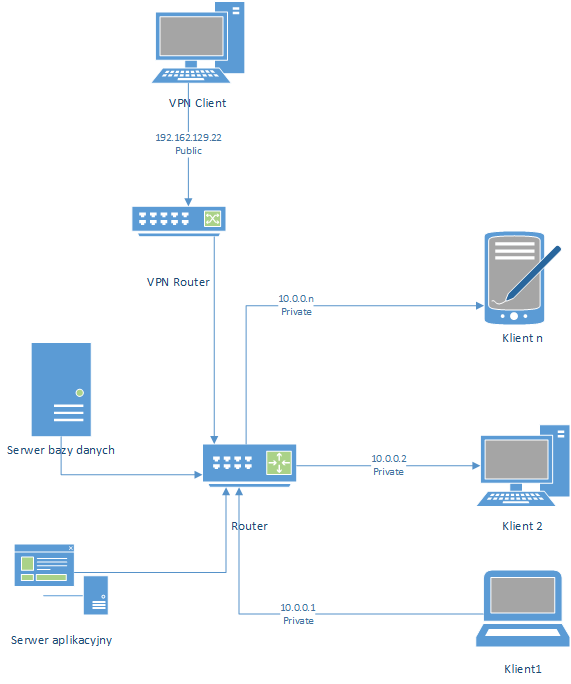
\includegraphics[scale=0.75]{deployment/siec}
    \caption{Schemat infrastruktury sieci}
    \label{fig:Deploymentdiagram1}
\end{figure}


\subsection{Specyfikacja technologii realizacji oprogramowania systemu}
System zostanie stworzony za pomocą wyszczególnionych w podrozdziale technologii.
\begin{enumerate}
	\item Aplikacja zostanie zrealizowana za pomocą technologii Java EE z użyciem frameworka Spring, który umożliwia tworzenie systemów zgodnie z architekturą MVC.
	\item Do przechowywania danych została wybrana relacyjna baza danych, aby zapewnić łatwe generowanie analiz. Zostanie zrealizowana w technologii Oracle Database 11g. Jednak interfejs aplikacji ma umożliwiać również zamiennie dołączanie bazy Postgres 9.4.
	\item Frontend aplikacji klienckiej zostanie zrealizowany w technologii HTML5, CSS 3.00 oraz JavaScript
	\item Aplikacja kliencka musi działać i być wyświetlana poprawnie pod przeglądarkami:
	\begin{itemize}
	 \item[-] Chrome (w wersji 8 i wyżej)
	 \item[-] Opera (w wersji 15 do wersji 19)
	 \item[-] Firefox (w wersji 29 do wersji 34)
	 \item[-] Internet Explorer (w wersji 8 i wyżej)
	 \end{itemize}
	\item Jako serwer webowy zostanie użyty GlassFish Server
\end{enumerate}

\begin{figure}[H]
    \centering
	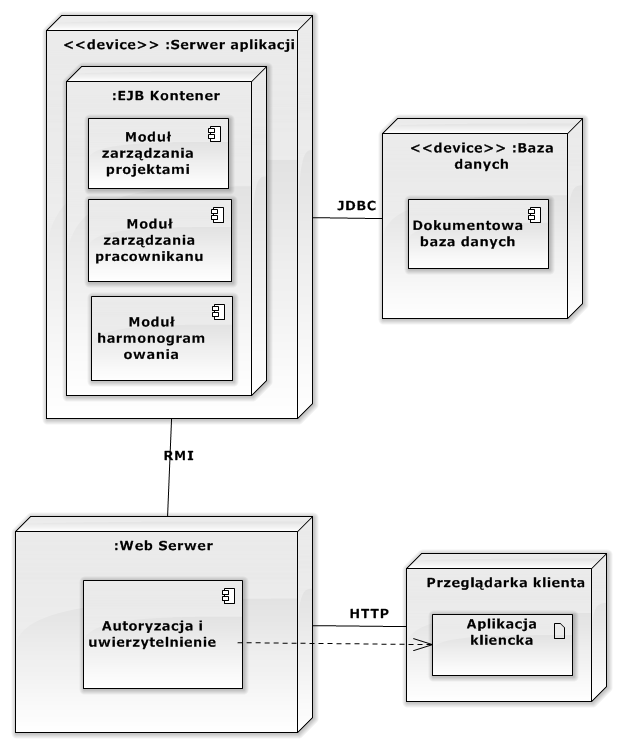
\includegraphics[scale=0.7]{deployment/Deploymentdiagram1}
    \caption{Schemat wdrożenia}
    \label{fig:Deploymentdiagram1}
\end{figure}

\subsection{Specyfikacja parametrów sprzętu}
Do stworzenia architektury zostaną użyte komputery o następujących parametrach:
\begin{itemize}
\item[-] Dell PowerEdge T320 with x8 HDD Backplane 
\item[-] Procesor - Intel Quad-Core Xeon E5-2403 (1.80 GHz, 10 M Cache, 6.4 GT/s QPI, 80W)
\item[-] RAM - 16GB DDR3 1333 MHz Dual Rank x4 LV RDIMM (2*8GB)
\item[-] Dysk twardy - 4x2TB 7200 rpm 3,5
\end{itemize}